This appendix documents the 30 fixed validation questions underlying \Cref{tab:validation-results}. The set covers five Korean corporate groups, with six questions per group: five selected-company briefings and one cross-company comparison. The versioned JSON artifacts retain the Korean prompts, expected claims, routing expectations, and answer checks.

\subsection{Validation Scenario Set}
\label{app:scenario-inventory}

The question design for each corporate group is summarized in \Cref{tab:question-design}.

\begingroup
\footnotesize
\setlength{\tabcolsep}{3pt}
\renewcommand{\arraystretch}{1.12}
\begin{longtable}{@{}C{0.12\linewidth}
                L{0.34\linewidth}
                L{0.25\linewidth}
                L{0.20\linewidth}@{}}
    \caption{Fixed validation-question design by corporate group.}
    \label{tab:question-design}\\
    \toprule
    \multicolumn{1}{C{0.12\linewidth}}{Corporate group} & \multicolumn{1}{C{0.34\linewidth}}{Differentiated question focus} & \multicolumn{1}{C{0.25\linewidth}}{Permitted evidence scope} & \multicolumn{1}{C{0.20\linewidth}}{Validation purpose} \\
    \midrule
    \endfirsthead
    \caption[]{Fixed validation-question design by corporate group (continued).}\\
    \toprule
    \multicolumn{1}{C{0.12\linewidth}}{Corporate group} & \multicolumn{1}{C{0.34\linewidth}}{Differentiated question focus} & \multicolumn{1}{C{0.25\linewidth}}{Permitted evidence scope} & \multicolumn{1}{C{0.20\linewidth}}{Validation purpose} \\
    \midrule
    \endhead
    \midrule
    \multicolumn{4}{r}{Continued on next page}\\
    \endfoot
    \bottomrule
    \endlastfoot
    Samsung & Semiconductor recovery, battery profitability, shareholder letter, biologics orders, insurance capital/dividend, and electronics--battery comparison. & DART financial data; official IR/DART narratives; financial affiliates limited to capital and dividend evidence. & Tests separation across electronics, battery, bio, construction, and financial-company evidence. \\
    SK & AI memory, battery restructuring, holding-company value-up, telecom AI/data centers, SK Square NAV/shareholder return, and Hynix--Innovation comparison. & DART financial data; value-up and shareholder-return material; source-backed operating-company and holding-company strategy claims. & Tests separation between operating-company, holding-company, and investment-company evidence. \\
    Hyundai Motor & Automaker, parts, logistics, defense/rail, and Hyundai Motor--Kia financial comparison questions. & DART annual financial data and business-mix claims tied to mobility and supply-chain affiliates. & Tests affiliate routing inside a closely related industrial supply chain. \\
    LG & Electronics, chemicals, battery, components, telecom financial trends, and electronics--chemicals comparison. & DART annual financial data and source-backed business-driver claims for heterogeneous sectors. & Tests whether the shared schema transfers across heterogeneous industries. \\
    Hanwha & Holding-company, aerospace, solar/materials, defense electronics, shipbuilding, and aerospace--solutions comparison questions. & DART financial data; official IR narratives; market and news interfaces only as traceable runtime signals when available. & Tests evidence contracts across defense, energy, systems, and shipbuilding topics. \\
\end{longtable}
\endgroup

Each group uses six questions: five selected-company briefings and one cross-company comparison. The columns specify question focus, permitted evidence scope, and validation purpose; a scenario set passes when routing, required claims, source links, follow-ups, and hidden-trace controls pass for all six questions. The prompts are translated for readability, with the original Korean prompts and expected claims stored in the scenario JSON files.

The table records design intent and links each question focus to the contract outcomes reported in \Cref{tab:validation-results}. Representative translated prompts are shown in \Cref{tab:question-examples}; the examples include briefing cards, market and filing signals, source links, follow-up questions, and bounded comparisons.

\subsection{Representative Question Examples}
\label{app:question-examples}

Translated examples of the fixed validation questions are given in \Cref{tab:question-examples}. The exact Korean prompts are stored in the versioned scenario JSON files. The examples vary the surface being exercised: news, market, filing, answer support, and bounded comparison.

\begingroup
\scriptsize
\setlength{\tabcolsep}{3pt}
\renewcommand{\arraystretch}{1.12}
\begin{longtable}{@{}C{0.19\linewidth}
                L{0.50\linewidth}
                L{0.22\linewidth}@{}}
    \caption{Representative fixed validation-scenario question examples.}
    \label{tab:question-examples}\\
    \toprule
    \multicolumn{1}{C{0.19\linewidth}}{Example type} & \multicolumn{1}{C{0.50\linewidth}}{Translated example question} & \multicolumn{1}{C{0.22\linewidth}}{Contract focus} \\
    \midrule
    \endfirsthead
    \caption[]{Representative fixed validation-scenario question examples (continued).}\\
    \toprule
    \multicolumn{1}{C{0.19\linewidth}}{Example type} & \multicolumn{1}{C{0.50\linewidth}}{Translated example question} & \multicolumn{1}{C{0.22\linewidth}}{Contract focus} \\
    \midrule
    \endhead
    \midrule
    \multicolumn{3}{r}{Continued on next page}\\
    \endfoot
    \bottomrule
    \endlastfoot
    Samsung selected company & Separate Samsung Electronics news, stock, and filing signals, then state what each source supports. & News, market, and filing separation \\
    SK selected company & Explain how the SK Hynix AI-memory brief is grounded and which follow-ups should be offered. & Affiliate routing and follow-up filtering \\
    Hyundai Motor selected company & Distinguish Hyundai Motor price movement from operating-performance evidence. & Market signal and filing evidence separation \\
    LG selected company & Summarize the LG Energy Solution battery-sector brief with source links and no unsupported forecast. & Source-link preservation and forecast restraint \\
    Hanwha selected company & Separate Hanwha Aerospace news and disclosure evidence before generating follow-up questions. & Evidence boundary and follow-up generation \\
    Cross-company comparison & Compare Hanwha Aerospace and Hanwha Solutions within promoted claims and source links. & Multi-entity routing and bounded comparison \\
    Answer-support check & After a finance brief, list source links and follow-up questions for reader inspection. & Reader-facing support controls \\
\end{longtable}
\endgroup

\subsection{Answer-Level Contract Examples}
\label{app:answer-contract-example}

The visible answer is part of the checked artifact. \Cref{tab:representative-answer-contract} summarizes representative output signals without reproducing full Korean transcripts; aggregate pass counts remain in \Cref{tab:validation-results}. Source links and follow-up questions are shown in \Cref{fig:representative-answer-output}.

\begingroup
\footnotesize
\setlength{\tabcolsep}{3pt}
\renewcommand{\arraystretch}{1.12}
\begin{longtable}{@{}C{0.12\linewidth}
                L{0.40\linewidth}
                L{0.24\linewidth}
                L{0.16\linewidth}@{}}
    \caption{Representative reader-visible answer signals across product surfaces.}
    \label{tab:representative-answer-contract}\\
    \toprule
    \multicolumn{1}{C{0.12\linewidth}}{Group} & \multicolumn{1}{C{0.40\linewidth}}{Representative visible output} & \multicolumn{1}{C{0.24\linewidth}}{Reader-facing support} & \multicolumn{1}{C{0.16\linewidth}}{Follow-up direction} \\
    \midrule
    \endfirsthead
    \caption[]{Representative reader-visible answer signals across product surfaces (continued).}\\
    \toprule
    \multicolumn{1}{C{0.12\linewidth}}{Group} & \multicolumn{1}{C{0.40\linewidth}}{Representative visible output} & \multicolumn{1}{C{0.24\linewidth}}{Reader-facing support} & \multicolumn{1}{C{0.16\linewidth}}{Follow-up direction} \\
    \midrule
    \endhead
    \midrule
    \multicolumn{4}{r}{Continued on next page}\\
    \endfoot
    \bottomrule
    \endlastfoot
    Samsung & Finance brief foregrounds margin recovery: 2024 revenue KRW 300.9T, operating income KRW 32.7T, and OPM 10.9\%; market-price evidence stays in the stock card. & DART filing, IR/filing package, KRX row, and news link remain visible to the reader. & Margin durability; debt and cash flow; shareholder return. \\
    SK & The visible answer separates SK Hynix AI-memory recovery from holding-company and investment-company questions, flagging HBM premium, CAPEX, and customer concentration as distinct variables. & Filing and IR links are exposed with selected claim evidence and source-state labels. & HBM CAPEX; customer exposure; SK Square NAV. \\
    Hyundai Motor & The output keeps stock movement as a market signal and operating performance as filing evidence, with sales mix, foreign exchange, hybrid/EV transition, and shareholder return treated as separate briefing axes. & KRX price row, OpenDART financial rows, and source links are shown as separate reader controls. & Hyundai--Kia comparison; margin resilience; parts and electrification. \\
    LG & The answer frames electronics cash flow separately from battery and chemical-cycle recovery, so margin defense and recovery timing are not collapsed into a single group-level statement. & OpenDART rows, IR/DART links, market rows, and unavailable-source states are labeled. & Battery cycle; LG Electronics margin; LG Chem recovery. \\
    Hanwha & Cross-company answers preserve the selected entities: aerospace, energy/materials, systems, and shipbuilding evidence are kept in bounded comparison rather than merged into one generic group brief. & DART, official IR, news, and market links are exposed where available with source-state labels. & Aerospace vs. Solutions; rights-issue evidence; disclosure risk signals. \\
\end{longtable}
\noindent These examples are condensed from generated answers: the table records the reader-visible signal, supporting evidence, and follow-up direction checked by the contract, while the full Korean answer text remains in the generated artifact.
\endgroup

\begin{figure}[H]
    \centering
    \makebox[\textwidth][c]{%
    \begin{minipage}[t]{0.49\linewidth}
        \centering
        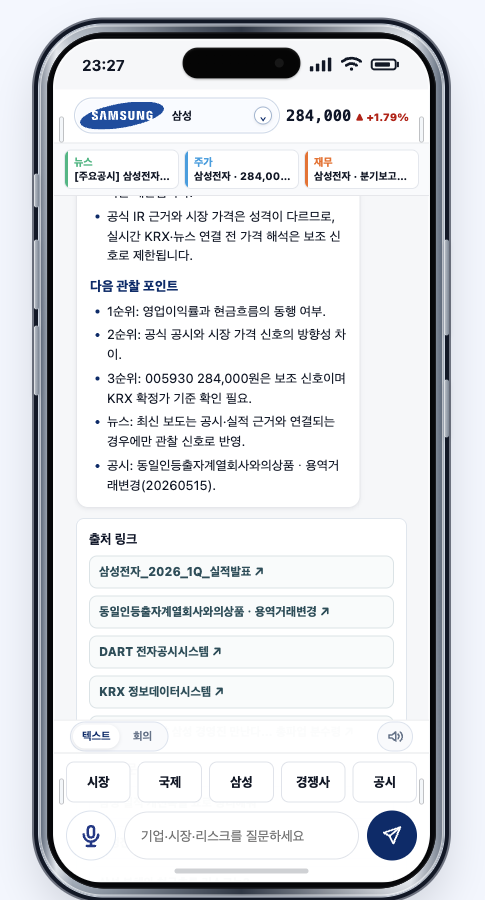
\includegraphics[width=\linewidth]{figures/ui_mobile_sources_ko.png}\\[-0.25em]
        {\small (a) Source links.}
    \end{minipage}
    \hspace{0.015\linewidth}
    \begin{minipage}[t]{0.49\linewidth}
        \centering
        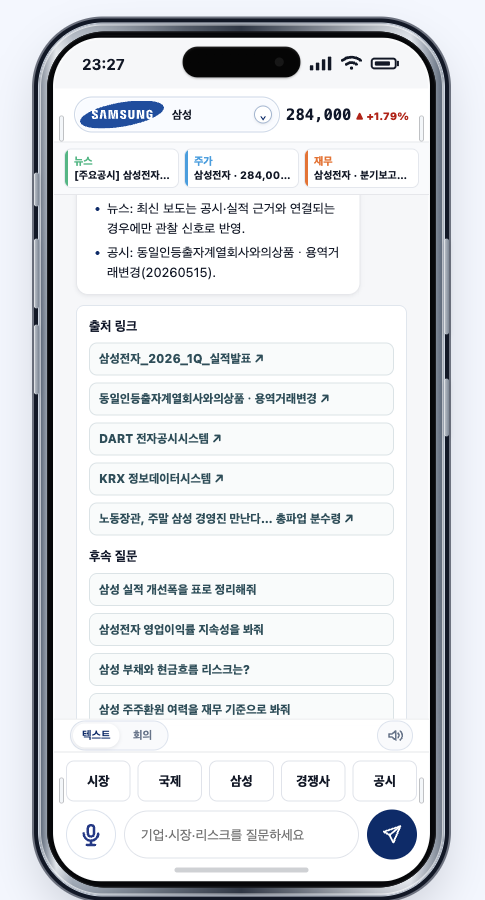
\includegraphics[width=\linewidth]{figures/ui_mobile_followups_ko.png}\\[-0.25em]
        {\small (b) Follow-up questions.}
    \end{minipage}}
    \caption{Representative answer-support screens in full mobile context. Panel (a) shows reader-facing source links; panel (b) shows generated follow-up questions, with internal trace details kept out of the visible answer.}
    \label{fig:representative-answer-output}
\end{figure}

\FloatBarrier

\subsection{Fault-Injection Protocol}
\label{app:fault-injection-protocol}

The fault-injection check induced seven contract violations, all of which were detected. \Cref{tab:fault-injection-protocol} lists the mutation rule and detected validator; the full JSON artifact is stored in \path{evals/results/} \citep{ahnkim2026advisorrepo}.

\begin{table}[H]
    \centering
    \small
    \setlength{\tabcolsep}{3pt}
    \renewcommand{\arraystretch}{1.12}
    \caption{Concrete mutation protocol for the fault-injection check.}
    \label{tab:fault-injection-protocol}
    \begin{tabular}{@{}C{0.18\linewidth}
                    L{0.25\linewidth}
                    L{0.37\linewidth}
                    C{0.13\linewidth}@{}}
    \toprule
    \multicolumn{1}{C{0.18\linewidth}}{Contract dimension} & \multicolumn{1}{C{0.25\linewidth}}{Baseline field mutated} & \multicolumn{1}{C{0.37\linewidth}}{Injected violation} & \multicolumn{1}{C{0.13\linewidth}}{Detected validator} \\
    \midrule
    Source claims & \path{sourceClaims} & Remove expected claim \texttt{samsung-sbc-020} from the source-claim package. & Claim coverage \\
    \bottomrule
    \end{tabular}
\end{table}

\begin{table}[H]
    \ContinuedFloat
    \centering
    \small
    \setlength{\tabcolsep}{3pt}
    \renewcommand{\arraystretch}{1.12}
    \caption[]{Concrete mutation protocol for the fault-injection check (continued).}
    \begin{tabular}{@{}C{0.18\linewidth}
                    L{0.25\linewidth}
                    L{0.37\linewidth}
                    C{0.13\linewidth}@{}}
    \toprule
    \multicolumn{1}{C{0.18\linewidth}}{Contract dimension} & \multicolumn{1}{C{0.25\linewidth}}{Baseline field mutated} & \multicolumn{1}{C{0.37\linewidth}}{Injected violation} & \multicolumn{1}{C{0.13\linewidth}}{Detected validator} \\
    \midrule
    Entity routing & \texttt{representative}\newline\texttt{CompanyId} and trace route & Replace \texttt{samsung-electronics} with an unrelated company identifier. & Trace contract \\
    Trace completeness & \path{trace.runId} & Delete a required trace field from the audit envelope. & Trace contract \\
    Answer contract & \path{answer} & Remove the required answer signal \textit{Samsung Electronics} from visible prose. & Answer contract \\
    Internal leakage & \path{answer} & Inject trace-schema labels and a raw source-claim identifier into the reader-facing answer. & Leakage gate \\
    Source links & \path{links[0].href} & Replace one source link with a non-resolving value, \texttt{not-a-valid-url}. & Link gate \\
    Latency budget & \path{elapsedMs} & Set elapsed time above the 1500ms pre-API latency budget. & Latency gate \\
    \bottomrule
    \end{tabular}
\end{table}
